\section{Experiment}

\subsection{Experiment Setup}

\subsubsection{Datasets}

We conduct experiments on the repartitioned Charades-CD and ActivityNet-CD~\cite{lan2022closer}. 
In these repartitioned datasets, the target moments of samples in the training, val, and test-iid sets are independent and identically distributed, while the test-ood set contains out-of-distribution samples. 
We can verify the debias ability of different models according to the grounding performance on the test-ood set and the performance difference between test-iid and test-ood sets.


\subsubsection{Metrics}
We use evaluation metrics of R@$n$, IoU=$m$, and mIoU. 
R@$n$, IoU=$m$ measures the proportion of test samples in which at least one of the top-$n$ localization results has an IoU score greater than $m$. 
The mIoU measures the average IoU score across all test samples. 
We set $n$ to 1 and $m$ to either 0.5 or 0.7, and use r1i5 and r1i7 to denote R@1, IoU=0.5 and R@1, IoU=0.7, respectively.
% We utilized the evaluation metrics of R$@n$, IoU=$m$ and mIoU. R$@n$, IoU=$m$ measures the percentage of testing samples with at least one localized result in the top-$n$ that has an IoU score greater than $m$ with the ground truth. On the other hand, mIoU measures the average IoU score across all testing samples. We use $n = 1$ and $m \in \{0.5,0.7\}$ in our experiments. We use r1i5 and r1i7 to respectively denote R@1, IoU=0.5 and R@1, IoU=0.7.


\subsubsection{Implementation Details}
For the text feature extractor, we use 300d GloVe~\cite{Glove} vectors for initialization. For the visual feature extractor, we use pre-trained I3D~\cite{I3D} and C3D~\cite{C3D} features. For the visual bias generator, we set $N_1$ to 4 and $M_1$ to 2. For the query bias generator, we set $N_2$ to 2 and $M_2$ to 4. During the training process, we use the AdamW~\cite{AdamW} optimizer, with a batch size of 16, and an initial learning rate of 0.001. We set $\lambda_{1}$ to 1, $\lambda_{2}$ to 1, and $\lambda_{3}$ to 1. 


\begin{table}[t]
	\centering
	% \small
	\renewcommand{\arraystretch}{1}
	\setlength{\tabcolsep}{1mm}
	\begin{tabular}{c|cc|ccc|ccc}
		% \hline
		\toprule
		\multirow{2}{*}{Row}
		& \multicolumn{2}{c}{BG} & \multicolumn{3}{c}{Grounding} &
		\multicolumn{3}{c}{OOD}  \\
		& $L_{loc}^g$ & $L_{cls}^g$ & $L_{loc}^d$ & $L_{cls}^d$ & $L_{kl}^d$
		& r1i5 & r1i7 & mIoU \\
		% \specialrule{1.5pt}{0em}{0em}
		\midrule
		1 & - & - & $\checkmark$ & - & - &
		43.08 & 22.52 & 41.52 \\
		2 & $\checkmark$ & - & $\checkmark$ & - & - &
		46.64 & 26.40 & 43.49 \\
		3 & $\checkmark$ & - & $\checkmark$ & - & $\checkmark$ &
		45.99 & 26.16 & 44.02 \\
		4 & - & $\checkmark$ & $\checkmark$ & $\checkmark$ & - &
		45.16 & 25.72 & 43.18 \\
		5 & - & $\checkmark$ & $\checkmark$ & $\checkmark$ & $\checkmark$ & 
		46.22 & 26.40 & 44.22 \\
		6 & $\checkmark$ & $\checkmark$ & $\checkmark$ & $\checkmark$ & - & 
		{\bf 47.41} & 26.84 & 44.00 \\
		7 & $\checkmark$ & $\checkmark$ & $\checkmark$ & $\checkmark$ & $\checkmark$ &
		47.20 & {\bf 27.17} & {\bf 44.59} \\
		\bottomrule
	\end{tabular}
	\caption{Ablation study about loss functions.}
	\label{loss term study}
	%\vspace{-3mm}
\end{table}


\subsection{Comparison with State-of-the-Arts}

To verify the universality of our debias strategy, we implement our BSSARD on multiple existing backbones QAVE, ExCL, and VSLNet*. The experiment results on Charades-CD and ActivityNet-CD datasets are presented in Table~\ref{sota-redivided}. 
We can see that our approach can significantly improve the grounding performance of different backbones on most evaluation metrics for OOD and IID test sets in both datasets. This indicates that our method has stronger debias and grounding ability. 
Besides, although our method shows the best performance in ActivityNet-CD's IID (BSSARD-VSLNet*), it works weaker than SVTG in Charades-CD's IID test set. This is due to the IID test set of Charades-CD containing a higher proportion of biased samples. 
% For example, in Charades-CD, our method achieves 4.12\% and 2.79\% for IoU=0.5, and 4.65\% and 1.46\% for IoU=0.7, respectively. Similarly, in ActivityNet-CD, our method achieves 1.62\% and 1.6\% for IoU=0.5, and 1.72\% and 2.53\% for IoU=0.7, respectively. 


\subsection{Ablation Study}

We conduct abundant ablation studies on Charades-CD datasets over BSSARD-VSLNet* backbones. 

\subsubsection{Loss Terms}

We analyze the impact of each loss function and their combinations on the grounding performance. Table~\ref{loss term study} summarizes the results. 
We can see that each loss function has its validity, and the combination of generation and adversarial losses can further improve the grounding performance on the OOD test set. 
Besides, the $L_{kl}^d$ leads to performance improvements in most cases. However, the improvement is limited when $L_{cls}^d$ is not used. This is because $L_{kl}^d$ depends on the grounding model's attention to the bias features brought by $L_{cls}^d$.


\begin{table}[t]
	\centering
	%\small
	\renewcommand{\arraystretch}{1}
	\setlength{\tabcolsep}{0.4mm}
	\begin{tabular}{c c c c | c c c}
		\toprule
		\multirow{2}{*}{Method} & \multicolumn{3}{c}{OOD} & \multicolumn{3}{c}{IID}\\
		& r1i5 & r1i7 & mIoU & r1i5 & r1i7 & mIoU \\
		\midrule
		%		QAVE &    &    &    &    &    &    \\
		%		QAVE-Q &    &    &    &    &    &    \\
		%		QAVE-V &    &    &    &    &    &    \\
		%		ADTGN-QAVE &    &    &    &    &    &    \\
		QAVE & 37.84 & 19.67 & 38.45 & 47.63 & 29.28 & 44.17 \\
		QAVE-Q & 41.96 & 23.20 & 40.97 & 50.18 & 32.56 & 47.11 \\
		QAVE-V & 42.79 & 22.34 & 41.03 & 54.07 & 33.41 & 48.31 \\
		BSSARD-QAVE & \bf 44.47 & \bf 26.16 & \bf 42.95 & \bf 54.31 & \bf 37.67 & \bf 49.41 \\
		\midrule
		ExCL & 39.61 & 19.35 & 38.81 & 47.18 & 26.59 & 44.02\\
		ExCL-Q & 39.94 & 19.7 & 39.05 & 48.90 & 26.59 & 44.72 \\
		ExCL-V & 39.10 & 19.21 & 38.77 & 47.79 & 30.76 &  45.58 \\
		BSSARD-ExCL & {\bf 41.93} & {\bf 22.53} & {\bf 40.9} & \bf 50.00 & \bf 31.86 & \bf 46.47 \\
		\midrule
		VSLNet* & 43.08 & 22.52 & 41.52 & 52.86 & 34.87 &  48.23 \\	
		VSLNet*-Q & 44.86 & 25.30 & 42.91 & 53.10 & 33.78 & 49.13 \\
		VSLNet*-V & 45.16 & 25.48 & 44.04 & {\bf 55.89} & {\bf 36.57} &  {\bf 51.60}\\
		BSSARD-VSLNet* & {\bf 47.20} & {\bf 27.17} & {\bf 44.59} & 55.65 & 36.33 & 50.45 \\
		\bottomrule
	\end{tabular}
	\caption{Ablation study about bias generator.}
	\label{backbones_charades_cd}
	%\vspace{-3mm}
\end{table}


\begin{table}[t]
	\centering
	\renewcommand{\arraystretch}{1}
	\begin{tabular}{c c c c c}
		\toprule
		visual & language & r1i5 & r1i7 & mIoU\\
		\midrule
		before & before & {\bf 47.32} & 26.46 & 44.30 \\
		before & after & 47.20 & {\bf 27.17} & {\bf 44.59} \\
		after & before & 45.45 & 25.30 & 42.66 \\
		after & after & 46.67 & 25.90 & 43.69 \\
		\bottomrule
	\end{tabular}
	\caption{Ablation study about bias injection positions. ``before'' and ``after'' represent the injection position before and after the feature encoder, respectively.}
	\label{bias_injection_positions}
\end{table}


\subsubsection{Bias Generator}

We analyze the impact of visual and query bias generators on different backbones and show the results in Tables~\ref{backbones_charades_cd}.
*-V and *-Q refer to the backbone model that uses only visual and query bias generators, respectively. The results show that the visual and query bias generators are effective on all backbones, and the two generators complement each other. 
Besides, we find that the performance of VSLNet*-V is even better than BSSARD-VSLNet* on the IID test set. This is mainly due to two reasons, one is that the powerful cross-modality alignment ability of VSLNet* weakens the integration effect of the two bias generators, and the other is the presence of numerous language bias samples in the IID test set.


\subsubsection{Bias Injection Positions}

We explore the effect of bias feature injection positions. 
The injection position determines which features the bias generator needs to generate bias on and which parts of the grounding model need to complete debias task. 
For visual and language biases, we separately test the injection position before and after the feature encoder. The results are shown in Table~\ref{bias_injection_positions}. 
We can see that injecting the visual bias feature before the visual feature encoder and injecting the language bias feature after the language feature encoder is the most effective. 
This primarily depends on the distinct characteristics of vision and text data and the need for both accuracy and diversity in generated bias features. First, the intricate nature of video content
and the high-dimensional visual feature space pose serious challenges for the feature encoder that aims to map visual and textual features into a shared space for multi-modal feature alignment. Injecting visual bias before the feature encoder reduces the encoder’s learning complexity, enabling the model to differentiate real from synthesized visual features. Second, introducing language bias after the feature encoder helps the model better capture bias during the multimodal feature alignment stage. Third, multiple injection positions increase the diversity of generated bias features. 

Besides, we inject bias in the feature domain instead of the input data because it is more controllable to generate high-quality sample features. If we directly generate video samples, the generator should not only capture the bias information but also learn the original video representation, which greatly increases the learning difficulty. %Moreover, we use the pre-trained models with fixed parameters to extract features, which can preserve rich relationships in the data domain in the feature space. 


\begin{table}[t]
	\centering
	\renewcommand{\arraystretch}{1}
	\begin{tabular}{c c c c c}
		\toprule
		$z_p$ & concat & r1i5 & r1i7 & mIoU\\
		% Fusion method & r1i5 & r1i7 & mIoU\\
		\midrule
		$\mathbb{R}^{n}$ & $F_T,F_V$ & 46.40 & 26.40 & 44.07 \\
		
		$\mathbb{R}^{3 \times n}$ & $F_T,F_V$ & {\bf 47.20} & {\bf 27.17} & {\bf 44.59}\\
		
		$\mathbb{R}^{3 \times n}$ & $F_T,F_V,F_S$ & 46.70 & 26.28 & 44.15 \\
		
		\bottomrule
	\end{tabular}
	\caption{Ablation study about fusion method of $z_p$.}
	\label{fusion method}
\end{table}


\begin{table}
	\centering
	\renewcommand{\arraystretch}{1}
	\setlength{\tabcolsep}{2mm}
	\begin{tabular}{c c c c}
		\toprule
		Training strategy & r1i5 & r1i7 & mIoU \\
		\midrule
		alternate each epoch & 46.79 & 26.76 & 44.53 \\
		
		random each step & 45.81 & 25.84 & 43.81 \\
		
		alternate each step & {\bf 47.20} & {\bf 27.17} & {\bf 44.59}\\
		
		\bottomrule
	\end{tabular}
	\caption{Ablation study about training strategy.}
	\label{Training strategy}
\end{table}



\subsubsection{Fusion Method of $z_p$ in VBG}
We investigate the impact of different fusion methods between $z_p$ and visual features in VBG. 
Table~\ref{fusion method} summarizes the results on the OOD test set.
We test three fusion methods, 
(1) encoding the temporal position as $z_p \in \mathbb{R}^{n}$ and fusing it with the temporal stream $F_T$ and video stream $F_V$.
(2) encoding the temporal position as $z_p \in \mathbb{R}^{3 \times n}$ and fusing it with $F_T$ and $F_V$.
(3) encoding the temporal position as $z_p \in \mathbb{R}^{3 \times n}$ and fusing it with the $F_T$, $F_V$ and spatial stream $F_S$. 
The results demonstrate that the second method is the most effective.
This is because $z_p \in \mathbb{R}^{3 \times n}$ can better represent temporal position information, and only the time stream $F_T$ and video stream $F_V$ containing temporal information that can better utilize temporal position information.


\begin{figure*}[t]
	\centering
	\subfigure[``cook'' suggests the target moment starts at the video start.]{
		%\includegraphics[width=5cm]{images/motivation-case-1.jpg}
		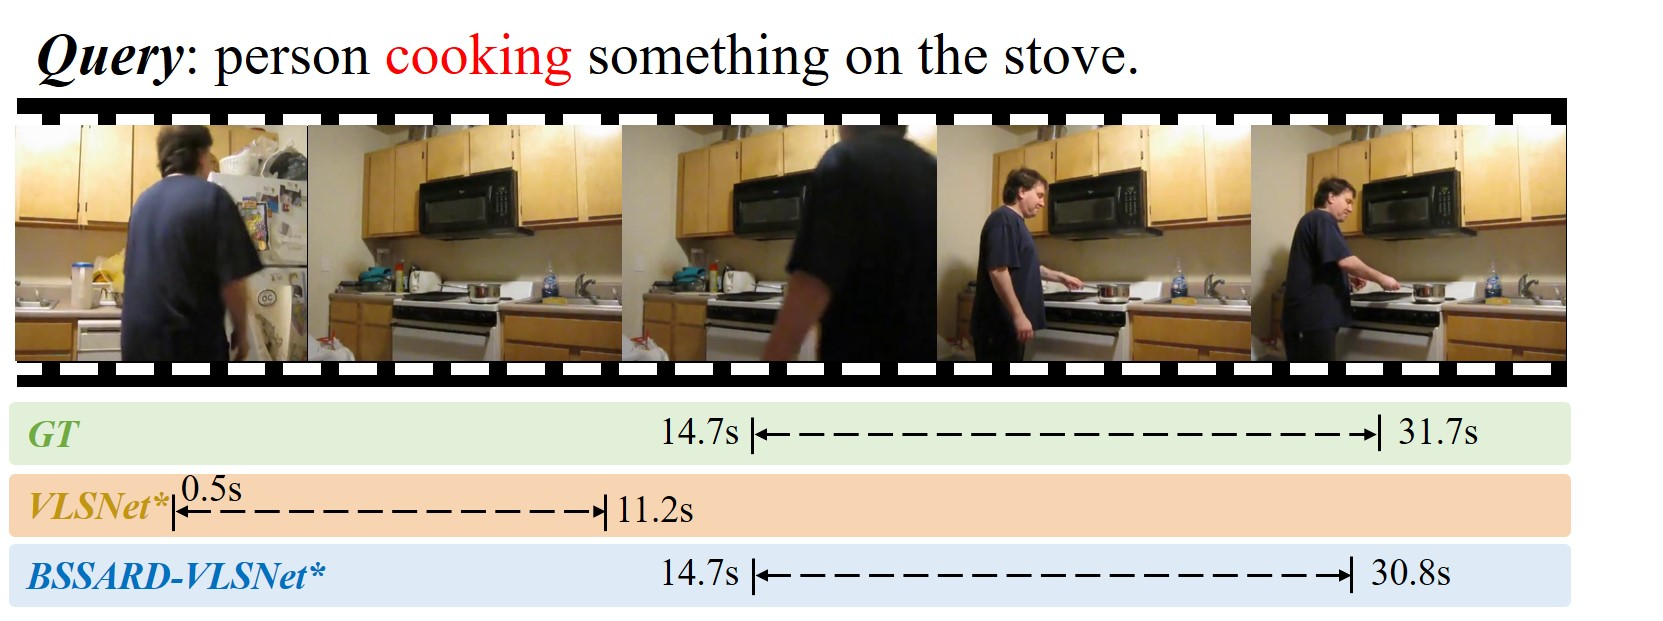
\includegraphics[scale=0.3]{images/cook.jpg}%-crop.pdf}
		\label{visualization_sample1}
	}
	\quad
	%\vspace{0.5mm}
	\subfigure[``start'' implies the target moment is at the end of the video.]{
		%\includegraphics[width=5cm]{images/motivation-case-2.jpg}
		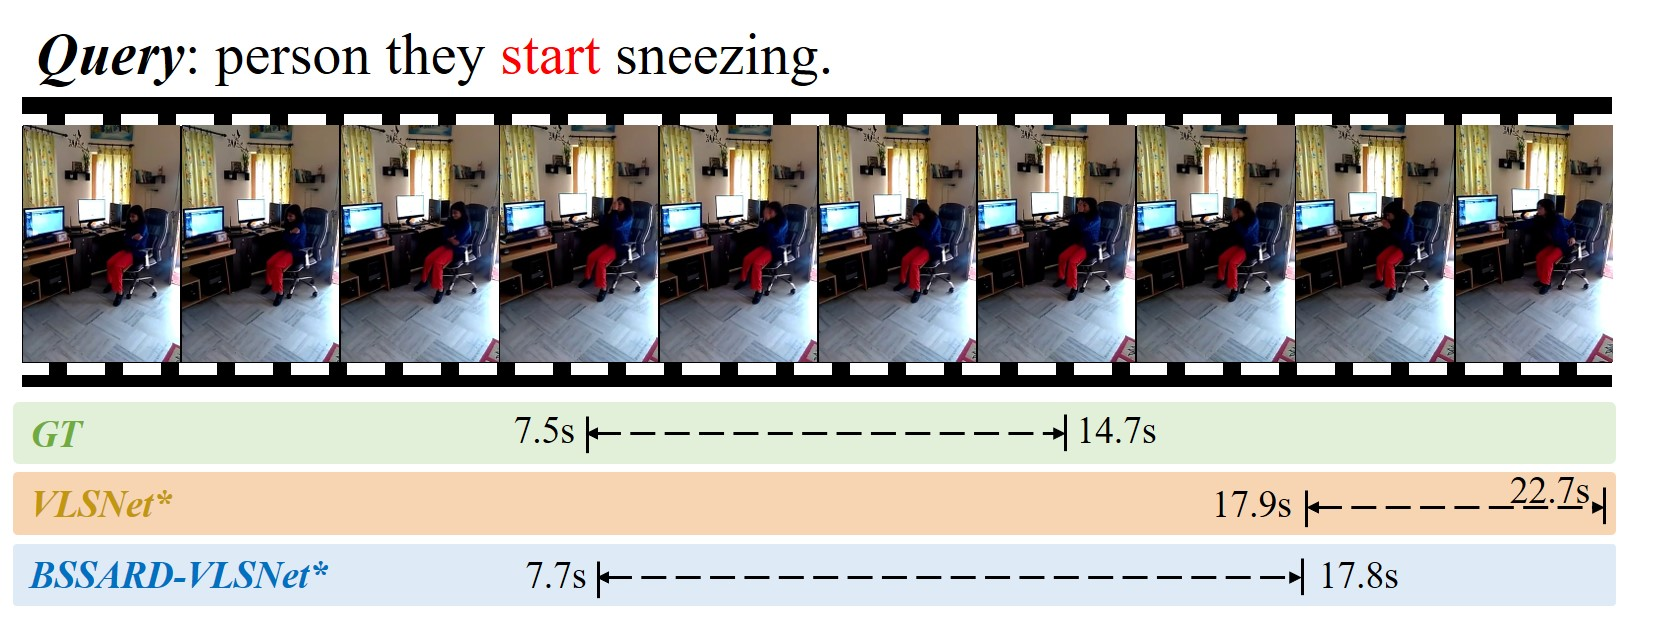
\includegraphics[scale=0.3]{images/start.jpg}%-crop.pdf}
		\label{visualization_sample2}
	}
	\quad
	\subfigure[``hold'' suggests the target moment starts at the video start.]{
		%\includegraphics[width=5cm]{images/motivation-case-3.jpg}
		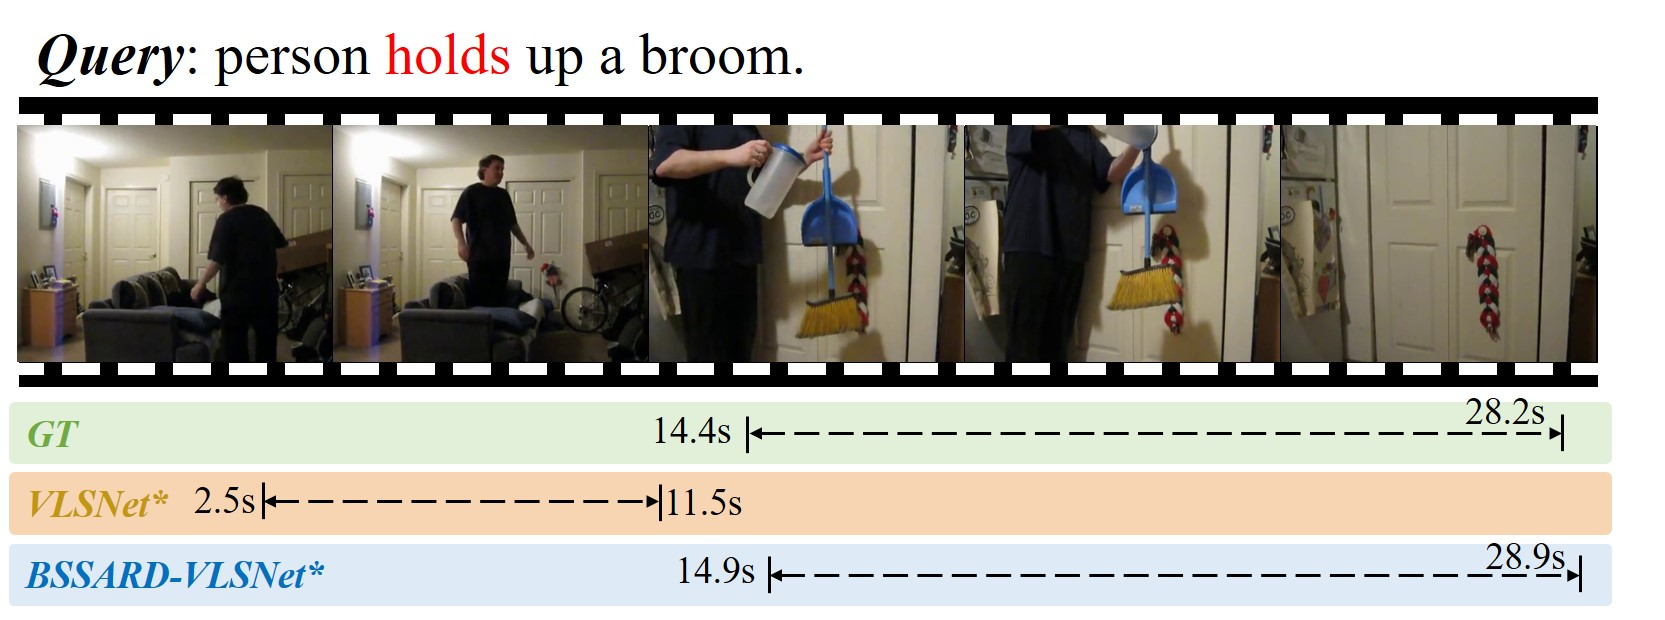
\includegraphics[scale=0.3]{images/hold.jpg}%-crop.pdf}
		\label{visualization_sample3}
	}
	\quad
	%\vspace{0.5mm}
	\subfigure[``hold'' suggests the target moment starts at the video start.]{
		%\includegraphics[width=5cm]{images/motivation-case-3.jpg}
		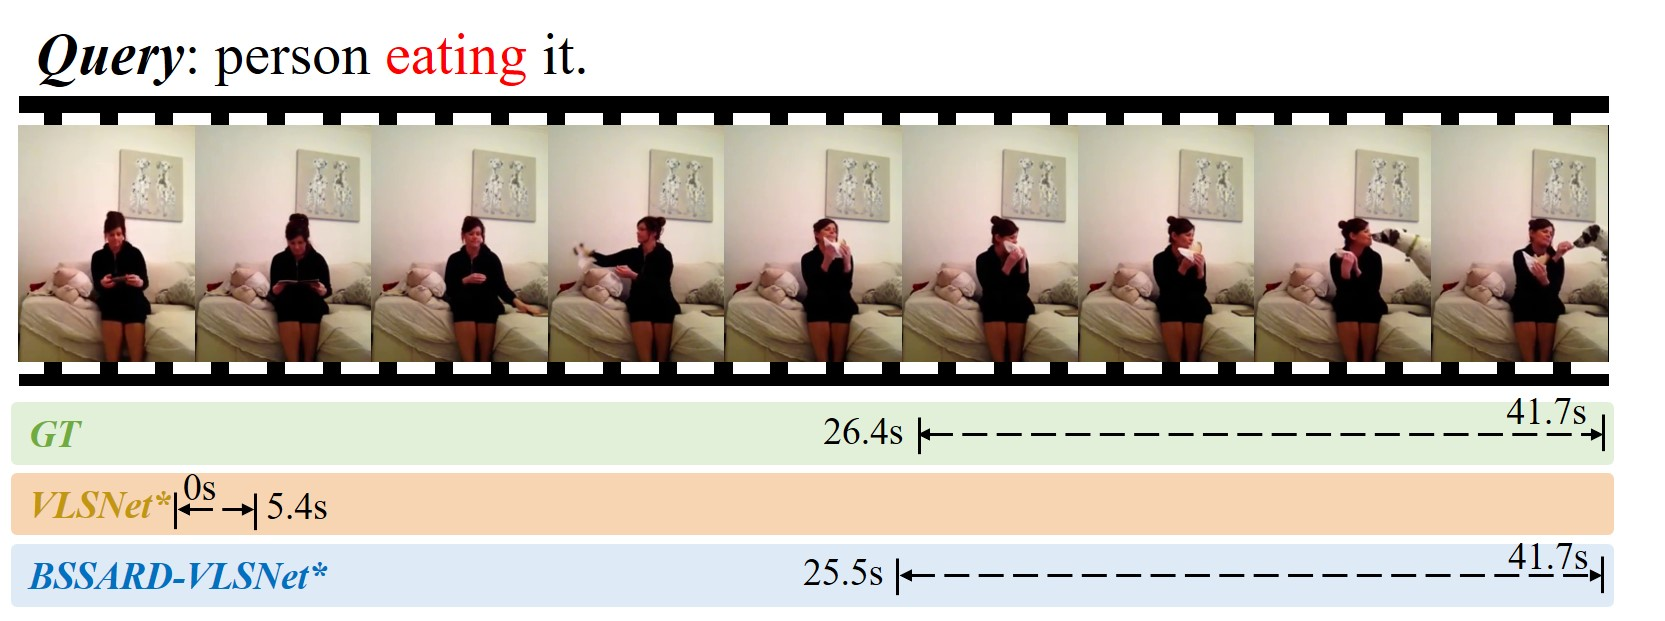
\includegraphics[scale=0.3]{images/eat.jpg}%-crop.pdf}
		\label{visualization_sample4}
	}
	\quad
	\centering
	\caption{The visualization comparison results between VLSNet* and BSSAR-VLSNet*.}
	\label{visualization_sample}
\end{figure*}


\subsubsection{Training Strategy for Bias Generators}
We investigate the impact of the training order of two bias generators and show results in Table~\ref{Training strategy}.
We test three training strategies: (1) alternately training the two bias generators at each epoch. (2) randomly selecting one bias generator for training at each training step. (3) alternately training the two bias generators at each training step. 
The experimental results indicate that the third training strategy is optimal. This is mainly because alternate training the two bias generators can avoid the model overfitting into a certain debias approach.


\subsection{Analysis of the Debias Effect}


\subsubsection{The Verification of Mitigating Bias} 

We randomly shuffle the words in each query text, which disrupts potential spurious correlations among query text and target moments. It also prevents the model from relying on visual-language alignment unless it depends on visual bias. Table~\ref{ablation_removing_language_bias} shows BSSARD achieves more significant performance degradation. This indicates our approach relies less on bias correlations beyond query text to perform grounding. 


\begin{table}[t]
	\centering
	\small
	\renewcommand{\arraystretch}{1}
	\setlength{\tabcolsep}{1.2mm}
	\begin{tabular}{c c c c c }
		\toprule
		Setting & B-VSLNet & VSLNet & B-QAVE & QAVE \\
		\midrule
		Original query & 47.20 & 43.08 & 44.47 & 37.84 \\
		%\midrule
		%Random video & 22.30 & 19.82 & 1.778 & 4.86 \\
		%Gap & \textbf{$\downarrow$ 52.75\%} & \textbf{$\downarrow$ 53.99\%} & \textbf{$\downarrow$ 96.00\%} & \textbf{$\downarrow$ 87.16\%} \\
		%\midrule
		Random query & 15.11 & 18.31 & 29.87 & 31.17 \\
		\midrule
		Gap & \textbf{67.99\% $\downarrow$ } & \textbf{57.50\% $\downarrow$} & \textbf{32.83\% $\downarrow$} & \textbf{17.63\% $\downarrow$} \\
		\bottomrule
	\end{tabular}
	\caption{Comparison results under random text input.}
	\label{ablation_removing_language_bias}
\end{table}


\subsubsection{Qualitative Analysis}

We also compare the debias effect of our BSSARD-VLSNet* and VLSNet* at the sample level in Figure~\ref{visualization_sample}. 
First, we give the temporal distribution of the target moment for samples with common verbs in the Charades-CD training set in Figure~\ref{sample_bias_distribution}. This indicates each verb contains prior knowledge for the localization of the target video clip. 
For example, the verb ``cook'' indicates that the temporal location of the target moments for most samples is the first half of the video. 
Hence, if the query text contains ``cook'' and the model will output the target moment with high probability in the first half of the video, which is the phenomenon of VLSNet* shown in Figure~\ref{visualization_sample1}. However, the result of our BSSARD-VLSNet* is not affected by the bias in the training set. 
The other three examples also show that the VLSNet* model relies on the bias in the training set for prediction, while our BSSARD-VLSNet* can effectively reduce the dependence on the bias and shift the model's attention back to cross-modality matching to make correct predictions. 


\begin{figure}[t]
	\centering
	{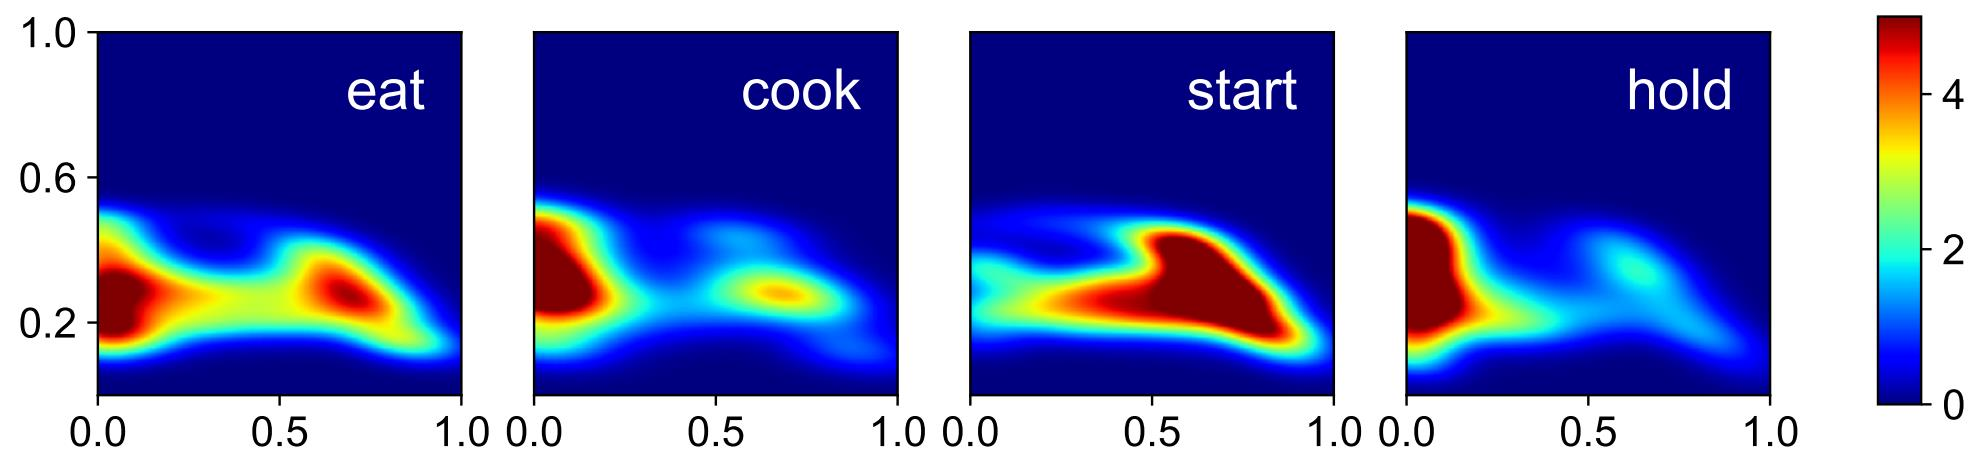
\includegraphics[width=1\linewidth]{images/distribution_four_word.jpg}}%.pdf}}
	\caption{The temporal distribution of target moments for video-text samples with certain common verbs. The horizontal and vertical axes denote the normalized starting time and duration of the target moment, respectively. The color represents the sample density.}
	\label{sample_bias_distribution}
\end{figure}
